\let\QuantumKernelLabel\label
\documentclass[a4paper,11pt,twocolumn,unpublished]{quantumarticle}
\pdfoutput=1
% Preserve the current LaTeX label hook across the class's older ltxutil layer.
\let\label\QuantumKernelLabel
\usepackage[T1]{fontenc}
\usepackage[utf8]{inputenc}
\usepackage{amsmath,amssymb,amsthm,mathtools}
\usepackage{tikz,pgfplots}
\usetikzlibrary{arrows.meta,positioning,calc}
\pgfplotsset{compat=1.18}
\renewcommand{\topfraction}{.9}
\renewcommand{\bottomfraction}{.9}
\renewcommand{\textfraction}{.05}
\setcounter{topnumber}{4}
\setcounter{totalnumber}{5}
\usepackage{microtype}
% quantumarticle uses the standard caption layout with a small sans-serif font.
\makeatletter\def\caption@documentclass{standard}\makeatother
\usepackage[font={small,sf},labelfont=normalfont,labelsep=colon]{caption}
\usepackage[numbers,sort&compress]{natbib}
\usepackage{hyperref}
\newtheorem{theorem}{Theorem}
\newtheorem{corollary}{Corollary}[section]
\newtheorem{lemma}{Lemma}[section]
\DeclareMathOperator{\cl}{cl}
\DeclareMathOperator{\capn}{cap}
\DeclareMathOperator{\Tr}{Tr}
\DeclareMathOperator{\supp}{supp}
\DeclareMathOperator{\Span}{span}
\newcommand{\ket}[1]{\lvert #1\rangle}
\newcommand{\bra}[1]{\langle #1\rvert}
\newcommand{\ddbar}[1]{\overline{\overline{#1}}}
\newcommand{\eps}{\varepsilon}
\newcommand{\EW}{\mathbb E_w}
\newcommand{\drec}{d_{\mathrm{rec}}}
\newcommand{\arxivref}[1]{\href{https://arxiv.org/abs/#1}{arXiv:#1}}
\title{From information tasks to exclusivity and Bell bounds}
\author{Samuel Mausberg}
\affiliation{Independent Researcher}
\date{3 October 2026}
\begin{document}
\maketitle
\begin{abstract}
Can possible information tasks explain the quantum bound on Bell correlations? We obtain a conditional bound, without assuming a quantum state space, and identify the additional task requirements that recover the quantum value. Homogeneous frequency limits and common calibration domains imply consistent exclusivity. Completing two-copy parity measurements with an ``other'' outcome gives a Bell bound controlled by the weights of these residual records. Marletto's T2 supplies four aligned parity sectors. A missing domain then requires an extra distinguishable label. An upper bound on readable labels, stable under adjoining spectators, and a reversible setting interchange remove the residual records. No-hypersignaling supplies this capacity bound when the relevant preparations are accessible and local signaling dimensions match the label counts. The result separates measurement existence, domain coverage, and readout weights.
\end{abstract}

\section{Introduction}
A Bell experiment has two separated laboratories, each choosing between two binary measurements. Quantum theory bounds the Clauser--Horne--Shimony--Holt (CHSH) correlation expression by $2\sqrt2$, although its algebraic maximum is four. Can constructor theory explain the smaller number through laws about possible and impossible information tasks \cite{cti,ctp}? We prove a conditional bound and isolate what its domain premise must accomplish. The issue is not the existence of a discriminator for joint parity labels. It is whether those labels cover the preparation used in the experiment.

The answer can be stated operationally. Add an ``other'' record to each of the aligned and crossed two-copy parity discriminators. If their respective weights are $\eps_0$ and $\eps_1$, then our task premises imply
\begin{equation}\label{eq:headline}
 B^2\leq 8+4(\eps_0+\eps_1)+288\kappa,
\end{equation}
where $\kappa$ bounds discrepancies between readouts with the same calibration. Homogeneous frequency tasks make $\kappa$ vanish. Parity-domain coverage makes both residual records vanish. Equation~\eqref{eq:headline} then gives the sharp quantum bound, with no quantum state space in the proof.

The result also gives a way to test the missing domain condition. T2 supplies four distinguishable aligned parity sectors. If there is no room for an additional distinguishable label, these sectors cover the substrate. The same argument must remain valid when another system---a spectator---is attached. A reversible task interchanging the two tested settings then supplies crossed coverage. We prove this capacity criterion, but do not derive its full-substrate capacity bound or setting interchange from T2.

A pair of qubits provides a running example. Fix the second qubit to $\ket+ = (\ket0+\ket1)/\sqrt2$ and leave the first unspecified. The sign of the second qubit is a perfectly readable and copyable label, yet the frequencies of the total computational-bit measurement depend on the first qubit. Specifying the preparation resolves that ambiguity. On two completely specified qubits, the four Bell labels exhaust the distinguishable information and jointly record two parities. These are different requirements: a frequency domain must be homogeneous, while a parity domain must be large enough.

We present three results. The first turns an operational frequency condition into calibrated weight neutrality and consistent exclusivity (CE). The second proves Eq.~\eqref{eq:headline} by keeping the residual records in Cabello's two-copy construction \cite{cabello}. The third expresses parity coverage as a consequence of information-capacity saturation and a reversible setting-interchange task. The proofs allow arbitrary state-space dimension and do not use an inner product, local tomography, or a rule assigning Born probabilities.

\begin{figure}[!htbp]
\centering
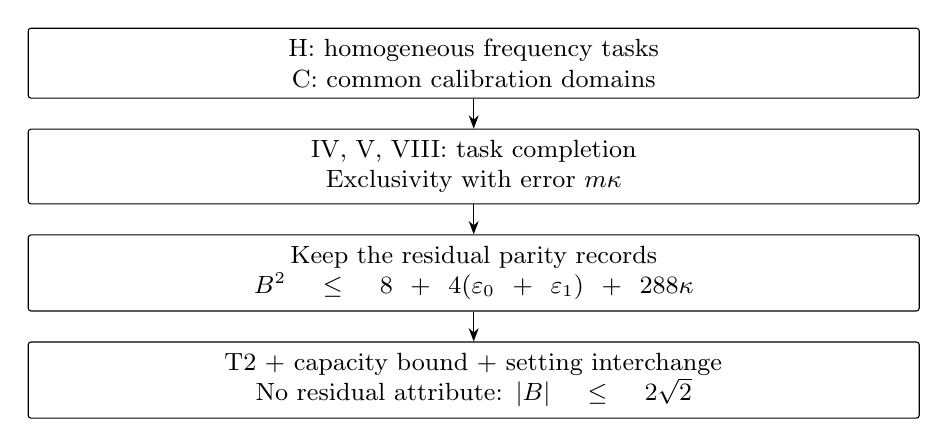
\begin{tikzpicture}[node distance=3.8mm,box/.style={draw,rounded corners=1pt,text width=.91\columnwidth,align=center,inner sep=4pt,font=\small},>=Stealth]
\node[box] (a) {H: homogeneous frequency tasks\\C: common calibration domains};
\node[box,below=of a] (b) {IV, V, VIII: task completion\\Exclusivity with error $m\kappa$};
\node[box,below=of b] (c) {Keep the residual parity records\\$B^2\leq8+4(\eps_0+\eps_1)+288\kappa$};
\node[box,below=of c] (d) {T2 + capacity bound + setting interchange\\No residual attribute: $|B|\leq2\sqrt2$};
\draw[->] (a)--(b);\draw[->] (b)--(c);\draw[->] (c)--(d);
\end{tikzpicture}
\caption{The three steps, under the record-weight and composition conventions of Sec.~2. H and C connect task calibration to weights. Completing a joint parity discriminator retains a possible residual record, whose weight appears in the Bell bound. Capacity saturation and reversible setting interchange remove it.}
\label{fig:logic}
\end{figure}

The relation between nonlocal states and joint measurements is established prior work. Short and Barrett identify the trade-off in boxworld \cite{short}. Czekaj, Horodecki, and Tylec constrain correlations by adding a Bell measurement \cite{czekaj}. Cabello's extra two-copy contexts supply our final counting argument \cite{cabello}. The contribution here is a finite-resolution connection from task calibration to weights, a bound retaining unresolved-domain records, and a distinguishable-label certificate for those domains.

The last certificate has a precise relation to no-hypersignaling \cite{hs}. Recording distinct labels is a narrower task than simulating every prepare-and-read distribution. We show how no-hypersignaling implies the needed capacity bound when local signaling dimensions match the available label counts and the witnessing attributes are preparable. An exact comparison with the published hypersignaling model shows why those qualifications matter. Section~7 places these results against sharpness, exclusivity, and parity-reading approaches.

\section{Tasks, preparations, and decision weights}
Locators for Refs.~\cite{cti,ctp} refer to arXiv versions v2 and v3, respectively, using their printed page numbers and named conditions. In particular, a condition on a selected observable is not a condition on every laboratory setting.

\subsection{The task principles used}
An attribute is a set of states. A task specifies an output attribute for every legitimate input attribute, and must work throughout that input set \cite[Sec.~2, pp.~8--11]{ctp}. We write $a\perp b$ when a possible discrimination task distinguishes them. Possible means arbitrarily accurately achievable, with no finite bound on the required accuracy \cite[Sec.~2, p.~8]{cti}. Distinguishability is symmetric, is inherited by subsets, and no nonempty attribute is distinguishable from itself.

The information principles are imposed on every finite composite. Interoperability allows independent information variables and their records to be combined; generic resources and task composition allow finite recording and counting networks \cite[Sec.~6, III, VI, VII, pp.~12--14]{cti}. Principle IV supplies a common discriminator for any finite pairwise distinguishable variable. Principle V upgrades statewise distinguishability to distinguishability of the whole attribute \cite[Sec.~6, p.~13]{cti}. Thus, with $\Omega$ the state set of the substrate,
\begin{equation}\label{eq:bar}
 \overline a=\{s\in\Omega:\{s\}\perp a\},\qquad \cl(a):=\ddbar a
\end{equation}
is an orthogonality closure. An observable attribute is closed under this operation. We use the finite-task portion of the information principles. Principle IX concerns ensemble discrimination and is not needed in these finite constructions \cite[Sec.~6, p.~19]{cti}. The local-description condition II is not identified with operational local tomography \cite[Sec.~2, p.~12]{ctp}.

For a finite measurable variable $X=\{x_i\}$, let
\begin{equation}\label{eq:domain}
 D_X=\cl\!\left(\bigcup_i x_i\right).
\end{equation}
A measurer is calibrated by the task $x_i\mapsto\text{record }i$. Nonperturbation, when required, means retention of the input attribute, not preservation of every compatible readout \cite[Sec.~5, Eqs.~(4)--(5), pp.~11--12]{cti}. Principle VIII says that all measurers of $X$ agree on every sharp output on $D_X$ \cite[Sec.~6, p.~16]{cti}. Its observable-closure consequence is that a coarse detector for an outcome $x_i$ is sharp on $\cl(x_i)$ \cite[Sec.~6, pp.~16--18]{cti}. Appendix~\ref{app:closure} states the precise completion properties we use.

These premises do not require a stochastic dynamics. We use ideal readouts in the task-accuracy closure: their record weights are limits of attainable readouts, and finite compositions and postprocessings respect these limits. This is an explicit accuracy convention, not an assertion that perfect constructors physically exist. The source asks subsidiary theories to provide suitable approximation structure \cite[Sec.~2, principle I, p.~12]{ctp}; the operational choice below is additional. When transporting attributes through a physical implementation, we represent it by a total transformation; its action outside the task's calibration inputs is otherwise unconstrained. This is also part of our operational convention. A finite operational representation of arbitrary dimension is sufficient, but the proofs do not require one.

\subsection{The record-weight bridge}
For a readout $M$, its record $i$, and a completely specified preparation $\omega$, write $w(M,i\mid\omega)$ for the derived decision weight. Weights are nonnegative and normalized. A sharp record has weight one, and grouping records adds their weights. Parallel repetition on independent instances has the same single-instance marginal weights. In the two-copy Bell argument, we also require
\begin{equation}\label{eq:product}
 w(e,e'\mid\omega\otimes\omega)=w(e\mid\omega)w(e'\mid\omega)
\end{equation}
for independently prepared experiments. This is Cabello's product premise \cite[step I, Eq.~(4)]{cabello}. These finite-record rules are explicit bridges. Nonsignalling alone does not supply the product rule.

We interpret these numbers as the values of zero-one games played on the final records \cite[Secs.~6--7]{ctp}. In particular, measurement neutrality P4 identifies the values of different implementations of the same game \cite[Sec.~7.2, p.~37]{ctp}. Its scope is important: T1/T2 select observables, rather than asserting a decision-weight extension for every possible readout. We assume the finite-record calculus on the calibrated networks used below. Theorem~\ref{thm:frequency} gives a second, quantitative route to their implementation independence; it does not rederive the whole decision-theoretic representation theorem.

Define an operational pseudometric on preparations of a fixed substrate by
\begin{equation}\label{eq:metric}
 d(\omega,\sigma)=\sup_{M\ \mathrm{binary}}\bigl|w(M,1\mid\omega)-w(M,1\mid\sigma)\bigr|.
\end{equation}
The supremum includes finite ancillary networks and their ideal readout limits. Distance to an attribute is the infimum over its members; for an empty attribute we set it to one. We make no use of the converse assertion that a weight-one outcome must be sharp.

\subsection{A finite-resolution repair of T1}
Condition E2 asks for one frequency partition on each qualifying attribute; T1 applies it to a selected observable and its two-copy sum \cite[Sec.~5, E2, p.~28; Sec.~6, T1, p.~30]{ctp}. Our domain consists instead of complete preparation instructions, specified independently of a measurement's weights. A coarser attribute is included only when the same limit works uniformly for all its preparations.

Here is the operational version of the limit. For a binary measurable variable $X=\{x_0,x_1\}$ and $L$ copies, form all sharp strings $x_{s_1}\otimes\cdots\otimes x_{s_L}$. For a candidate frequency $f\in[0,1]$ and resolution $h>0$, define
\begin{equation}\label{eq:window}
 A_{X,L}(f,h)=\cl\!\bigcup_{\substack{s\in\{0,1\}^L\\|L^{-1}\sum_j s_j-f|\leq h}}
 x_{s_1}\otimes\cdots\otimes x_{s_L}.
\end{equation}
The union is a calibration attribute for the task that counts the ones and reports whether their frequency lies in the window. By VIII, every implementation of that counting task reports yes sharply on its closure. Thus Eq.~\eqref{eq:window} is defined by attributes and tasks, not by choosing an apparatus's output distribution.

\paragraph{Operational homogeneity H.}
For every complete preparation $\omega\in D_X$ and every binary comparison variable used in the proof, including those generated by discrimination completion, there is one $f$ such that, for each fixed $h>0$,
\begin{equation}\label{eq:H}
 \delta_{X,L}(\omega;f,h):=d\bigl(\omega^{\otimes L},A_{X,L}(f,h)\bigr)\longrightarrow0.
\end{equation}
H makes two additions to a mere restriction of T1's domain. It chooses the operational topology for the frequency limit, and extends the frequency condition to the finite family of tested binary coarse-grainings. Neither addition is attributed to the printed T1. A law of large numbers for one chosen apparatus is weaker than H.

Quantum preparations satisfy H for projective variables: projection onto a frequency window gives a nearby input on which that window is sharp. Appendix~\ref{app:frequency} proves
\begin{equation}\label{eq:qH}
 \delta_{X,L}(\rho;f,h)\leq\min\left\{1,\frac{1}{2h\sqrt L}\right\}.
\end{equation}
This is a consistency example only. The main theorems use Eq.~\eqref{eq:H}, not quantum projection.

\subsection{Compositional calibration coverage}
A record-producing circuit is not automatically a measurer of an input information variable. We therefore state its required coverage separately.

\paragraph{Coverage C.}
For the finite experimental scenario, there is one enlarged substrate obtained by appending fixed independent finite ancillas. Each tested context is a calibrated measurer of a finite information observable on that substrate, possibly followed by classical coarse-graining. The common enlarged preparation belongs to every corresponding domain $D_X$. The identifications of local calibration attributes persist when spectators are appended, so that a shared local setting with opposite records defines distinguishable global calibration attributes. The same condition holds for the finite independent copies used in the experiment.

In the capacity argument we also use independent calibration resources: the calibration attributes in its finite frames admit nonempty independent products, and their local discriminators retain their calibration on those products. Appending any fixed member is an available total preparation map. This specifies the product-input convention used with III and VI, without imposing a numerical factorization on correlated inputs.

This is a task statement about calibration, domains, and composition. It does not require a postmeasurement instrument to preserve compatible statistics. It is therefore not Chiribella--Yuan fundamental sharpness, although their dilation premise is a relevant stronger operational motivation \cite[Principle 1 and the reduction to sharp measurements]{sharp}. The distinction between allowed effects and specified measurement tasks is also central to restricted-effect theories \cite[Sec.~IV]{restricted}.

\section{From frequency limits to exclusivity}
Joint distinguishability alone supplies a new measurement, but says nothing numerical about its relation to existing readouts. The next theorem supplies that relation. Its proof concerns attributes and readout weights, without a state-space representation.

\begin{theorem}[Frequency-neutral task completion]\label{thm:frequency}
Assume the task principles and finite-record bridge of Sec.~2. Let $M,N$ be any two measurers of the same binary variable $X$, and let $\omega\in D_X$. For every $f,h,L$,
\begin{equation}\label{eq:neutral}
\begin{aligned}
 |w(M,1\mid\omega)-f|&\leq h+\delta_{X,L},\\
 |w(M,1\mid\omega)-w(N,1\mid\omega)|&\leq2h+2\delta_{X,L}.
\end{aligned}
\end{equation}
Under H, all such readouts have the same weights.

Consider finitely many covered events on one preparation, each represented by a closed outcome attribute of its context. If these attributes are pairwise distinguishable, their weights sum to at most one. More generally, if every comparison of calibrated binary measurers required in the completion differs by at most $\kappa$, a family of $m$ events obeys
\begin{equation}\label{eq:ce}
 \sum_{i=1}^m w(e_i\mid\omega)\leq1+m\kappa.
\end{equation}
Consequently H and C imply CE for covered events and local orthogonality (LO) at every finite-copy level. Product weights are needed only to identify independent-copy statistics with the usual hierarchy.
\end{theorem}
\begin{proof}
Repeat $M$ in parallel $L$ times, and call the record frequency $F$. Its mean weight is $w(M,1\mid\omega)$, by the marginal assumption. On a preparation in $A_{X,L}(f,h)$, the window detector is sharp. Equation~\eqref{eq:metric} therefore bounds its failure weight on $\omega^{\otimes L}$ by $\delta_{X,L}$. Since $0\leq F,f\leq1$, splitting the finite weighted sum into the window and its complement gives
\begin{equation}\label{eq:mean}
 |\EW F-f|\leq\EW|F-f|\leq h+\delta_{X,L}.
\end{equation}
The two estimates in Eq.~\eqref{eq:neutral} follow. Taking $L$ to infinity and then $h$ to zero proves neutrality. Independence among the $L$ records was not used.

For the completion, let $x_1,\ldots,x_m$ be the closed event attributes and put $r=\overline{\bigcup_i x_i}$. The nonempty members of
\begin{equation}\label{eq:completion}
 Z=\{x_1,\ldots,x_m,r\}
\end{equation}
are pairwise distinguishable. Their union has closure $\Omega$: its bar is $\overline{\bigcup_i x_i}\cap\cl(\bigcup_i x_i)$, which is empty. Principle IV supplies a common discriminator $D$.

Coarse-grain $D$ to ``$i$ or not $i$''. It is a measurer of the same binary calibration variable as a Boolean discriminator for $\{x_i,\overline{x_i}\}$. Applying VIII on the full domain shows that this coarse-graining is itself calibrated on that Boolean variable. It is therefore also a measurer of the binary coarse-graining of the original context that defines event $i$. The original preparation is in that context's domain by C. Neutrality identifies the two weights, or bounds their difference by $\kappa$. Summing the $m$ outcomes of $D$ proves Eq.~\eqref{eq:ce}.

For LO, two locally exclusive events differ in the outcome of the same local setting. That local readout distinguishes their global calibration attributes under C. The preceding completion applies to each finite set and to every finite composite. The independent-copy product rule gives the usual hierarchy. The closure and calibration details are proved in Appendix~\ref{app:closure}.
\end{proof}

The physical content is that possible discrimination must preserve the weights already assigned to its calibration labels. The theorem does not construct a minimally disturbing instrument. Its qualitative neutrality conclusion agrees with the game-level P4 of Ref.~\cite{ctp}; Eq.~\eqref{eq:neutral} gives a direct frequency estimate and identifies the input topology needed for that conclusion.

There is a second sufficient reading of the qualitative step. Suppose the zero-one games for every comparison variable in Appendix~\ref{app:closure} fall within the decision-supporting domain, and suppose P4 applies to their implementations. Appending the same reward adder to either calibrated detector implements the same game, so P4 identifies their values. Those values are the two event weights by the record-weight bridge. The completion proof then gives CE without invoking H. Extending the game domain to all these variables is an explicit premise; it is not supplied by citing P4 for one selected observable. The finite estimate in Eq.~\eqref{eq:neutral} remains an additional conclusion of H.

There is a useful converse certificate. If a family of $m$ pairwise distinguishable covered events has weight sum $1+\Delta$, with $\Delta>0$, at least one binary comparison in the completion differs by at least $\Delta/m$. For any proposed common frequency center,
\begin{equation}\label{eq:converse}
 \delta_{X,L}\geq\frac{\Delta}{2m}-h\qquad\text{for every }L.
\end{equation}
This obstruction is independent of local dimension and state-space geometry. It identifies a finite-frequency task that fails.

\section{The Bell bound with a residual record}
Exclusivity becomes useful for CHSH only when the additional parity events are represented by calibrated readouts. Instead of assuming that a joint parity variable covers the input, we complete it and retain the extra outcome. This makes the domain issue quantitative.

Let Alice and Bob have settings $x,y\in\{0,1\}$ and outcome bits $a,b\in\{0,1\}$, corresponding to signs $(-1)^a,(-1)^b$. Define
\begin{equation}\label{eq:chsh}
\begin{aligned}
 E_{xy}&=\sum_{a,b}(-1)^{a+b}w(a,b\mid x,y),\\
 B&=E_{00}+E_{01}+E_{10}-E_{11}.
\end{aligned}
\end{equation}
The doubled preparation is $\omega\otimes\omega$, on laboratories $(A,B,A',B')$. Fixed ancillas needed by C are included in the laboratory substrates.

For $t=0,1$, compare Alice's setting $x$ with Alice$'$'s setting $x\oplus t$. The choices $t=0$ and $t=1$ are called aligned and crossed. Let $U^c_{t,x}$ be the union of product calibration attributes with $a\oplus a'=c$, including arbitrary independent spectator preparations. On the full substrate define
\begin{equation}\label{eq:parities}
\begin{aligned}
 p^c_{t,x}&=\cl(U^c_{t,x}),\\
 h^{cd}_t&=p^c_{t,0}\cap p^d_{t,1},\qquad
 V_t=\bigcup_{c,d\in\{0,1\}}h^{cd}_t.
\end{aligned}
\end{equation}
The local readouts followed by a parity computation distinguish $U^0_{t,x}$ and $U^1_{t,x}$. VIII extends their sharp records to the closed sectors. Different nonempty $h^{cd}_t$ are therefore pairwise distinguishable. IV supplies a discriminator for the variable $H_t$ formed by these attributes. As throughout the paper, empty outcomes are omitted.

A discriminator need not have the required domain. Define its residual attribute and completed variable by
\begin{equation}\label{eq:paritycomplete}
 r_t=\overline{V_t},\qquad
 \widehat H_t=\{h^{cd}_t:h^{cd}_t\ne\varnothing\}\cup\{r_t\},
\end{equation}
again omitting $r_t$ if empty. The completion argument of Theorem~\ref{thm:frequency} gives $D_{\widehat H_t}=\Omega$. Choose one calibrated discriminator $\widehat J_t$ of this full-domain variable and put
\begin{equation}\label{eq:residual}
 \eps_t=w(\widehat J_t,r_t\mid\omega\otimes\omega).
\end{equation}
Set $\eps_t=0$ if $r_t$ is empty. Under H this number is independent of the calibrated implementation. It is an ordinary record weight, not a probability that the constructor malfunctions and not an assumed mixture fraction outside a subspace.

\paragraph{Parity-domain coverage P.}
The domain condition used in the zero-residual theorem is
\begin{equation}\label{eq:P}
 \omega\otimes\omega\in D_{H_t}=\cl(V_t),\qquad t=0,1.
\end{equation}
It is the task-domain counterpart of Cabello's joint-parity normalization assumption \cite[step III, Eq.~(5), and the extension to Eq.~(10)]{cabello}. Its formulation does not assign simultaneous values to the original local settings. P implies $\eps_0=\eps_1=0$: the residual detector is sharp no on $\cl(V_t)$. We will not use the converse assertion that a zero weight implies a sharp prediction.

\begin{theorem}[Residual-weight Bell bound]\label{thm:bell}
Assume the task principles, the finite-record bridge, and coverage C. Let $\kappa\geq0$ bound every calibrated binary comparison in the sixteen discrimination completions specified below. With independent-copy factorization,
\begin{equation}\label{eq:bell}
 B^2\leq8+4(\eps_0+\eps_1)+288\kappa.
\end{equation}
Under H, one may set $\kappa=0$. Under P as well, the consequence is
\begin{equation}\label{eq:tsirelson}
 |B|\leq2\sqrt2,
\end{equation}
and this constant is sharp. With P and finite calibration discrepancies,
\begin{equation}\label{eq:kappabell}
 B^2\leq8+288\kappa.
\end{equation}
More generally,
\begin{equation}\label{eq:distance}
 \eps_t\leq d(\omega\otimes\omega,D_{H_t}),
\end{equation}
so either residual weights or operational distances to the parity domains give valid error bounds.
\end{theorem}
\begin{proof}
Let $S$ be the sum of the eight weights satisfying the CHSH winning relation $a\oplus b=xy$. Normalization gives
\begin{equation}\label{eq:winning}
 S=2+\frac B2,\qquad
 \sum_{a\oplus b\ne xy}w(a,b\mid x,y)=4-S.
\end{equation}
For each $t,c,d,k\in\{0,1\}$, form eight four-laboratory events indexed by $x,a,b\in\{0,1\}$:
\begin{equation}\label{eq:generator}
\begin{aligned}
 x'&=x\oplus t,\quad y=k,\quad y'=k\oplus1\oplus c\oplus d,\\
 a'&=a\oplus1\oplus\gamma_x,\quad(\gamma_0,\gamma_1)=(c,d),\\
 b'&=b\oplus1\oplus\gamma_x\oplus xy\oplus x'y'.
\end{aligned}
\end{equation}
Adjoin the outcome $h^{cd}_t$ of $\widehat J_t$, unless it is empty. These are at most nine pairwise distinguishable closed event attributes. Within one $x$ block, different $(a,b)$ are locally exclusive. Between the blocks, $b\oplus b'$ changes while Bob's settings stay fixed, so at least one Bob record differs. Each fine event has Alice parity opposite to the $x$ component of $h^{cd}_t$.

Theorem~\ref{thm:frequency} bounds each event sum by $1+9\kappa$. Across the sixteen choices, every ordered winning--winning or losing--losing pair occurs exactly once, and each joint parity outcome occurs twice. Appendix~\ref{app:certificates} proves this using an explicit inverse to Eq.~\eqref{eq:generator}. Product factorization and normalization of the completed readouts now give
\begin{equation}\label{eq:sum16}
 S^2+(4-S)^2+2\sum_{t=0}^1(1-\eps_t)\leq16+144\kappa.
\end{equation}
Substitution of Eq.~\eqref{eq:winning} proves Eq.~\eqref{eq:bell}. H removes $\kappa$ by Theorem~\ref{thm:frequency}. P removes the two residual weights by their sharp-no calibration. The qubit construction in Appendix~\ref{app:quantum} attains equality.

Finally, the residual detector is zero on every preparation in $D_{H_t}$. Comparison with any such preparation in Eq.~\eqref{eq:metric}, followed by an infimum, proves Eq.~\eqref{eq:distance}. The empty-domain convention covers that case too.
\end{proof}

The only change to Cabello's numerical argument is retaining the two residual weights. Their presence identifies what is needed from the task domains. Figure~\ref{fig:bound} plots the resulting bound. A common frequency-window radius $h$ and distance bound $\delta$ in the binary comparisons replace the last term in Eq.~\eqref{eq:bell} by $576(h+\delta)$.

\begin{center}
\begin{minipage}{\columnwidth}
\captionsetup{hypcap=false}
\centering
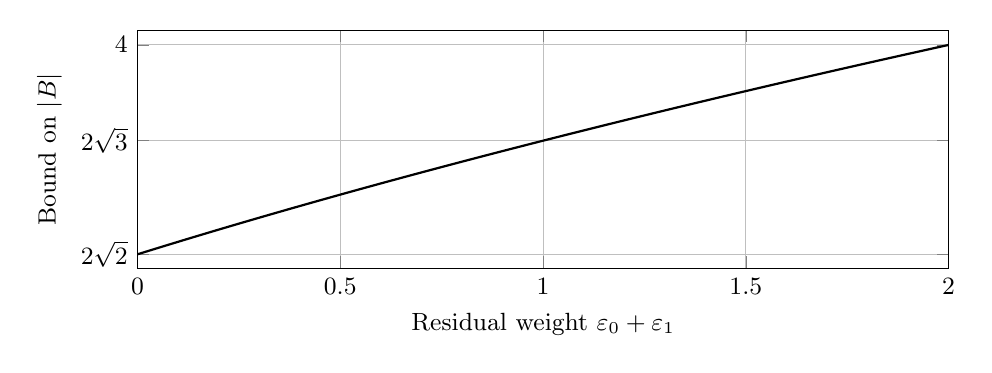
\begin{tikzpicture}
\begin{axis}[width=.98\columnwidth,height=4.6cm,xmin=0,xmax=2,ymin=2.75,ymax=4.08,
 xlabel={Residual weight $\eps_0+\eps_1$},ylabel={Bound on $|B|$},
 xtick={0,.5,1,1.5,2},ytick={2.8284271247,3.4641016151,4},yticklabels={$2\sqrt2$,$2\sqrt3$,$4$},
 tick label style={font=\small},label style={font=\small},grid=major]
\addplot[thick,domain=0:2,samples=101]{sqrt(8+4*x)};
\end{axis}
\end{tikzpicture}
\captionof{figure}{The residual-weight bound at $\kappa=0$: $|B|\leq\sqrt{8+4(\eps_0+\eps_1)}$. Zero residual weight gives $2\sqrt2$; no restriction on the residual records gives the algebraic bound four. Attainability is established at zero residual weight, not along the whole curve.}
\label{fig:bound}
\end{minipage}
\end{center}

\section{What T2 contributes: sectors and capacity}
The previous theorem reduces the Bell question to two calibrated residual records. To connect it to T2, we first construct the aligned sectors and then ask what would make their residual attribute empty. The relevant task notion is the number of distinguishable information labels, not the number of state coordinates.

\subsection{The four aligned sectors}
Let $S_A$ denote Alice's active substrate and let $X=\{x_0,x_1\}$ and $Y=\{y_0,y_1\}$ be the binary sector selected by T2. The source's labels $x_1,x_2,y_+,y_-$ have only been relabelled. R1 places these attributes in the required generalized-mixture relations. R2 supplies label flips that preserve the other variable's attributes. R3 identifies specified intrinsic measurement attributes. R4 supplies a two-copy generalized mixture $q$ of the equal-$X$ products and of the equal-$Y$ products \cite[Sec.~6, T2, R1--R4, pp.~30--32]{ctp}.

On $S_A\otimes S_A$, use the same parity definition as Eq.~\eqref{eq:parities}, without spectators for now. R2 and R4 imply that all four aligned sectors are nonempty. Indeed, write $T_X$ for the R2 operation on the first copy that flips $x_0,x_1$ while preserving both $y$ attributes, and $T_Y$ for its counterpart. Then
\begin{equation}\label{eq:four}
\begin{aligned}
 q&\subseteq h^{00}_0,& T_Xq&\subseteq h^{10}_0,\\
 T_Yq&\subseteq h^{01}_0,& T_XT_Yq&\subseteq h^{11}_0.
\end{aligned}
\end{equation}
Appendix~\ref{app:transport} proves that possible total transformations transport distinguishability closure, which justifies these inclusions without assuming globally reversible label flips. All four attributes are pairwise distinguishable. R1 and R3 remain conditions on a T2 theory, but are not used in this sector-construction lemma.

\subsection{A task certificate for an exhaustive domain}
For a substrate $S$, let $\capn(S)$ be the greatest number of nonempty pairwise distinguishable attributes it admits, when finite. IV turns every such family into a common discrimination task; call the family a frame. Thus an upper bound on $\capn(S)$ is an impossibility statement about recording too many mutually distinguishable input labels. It is not a bound on the dimension of an operational state space.

Deutsch and Marletto call a variable maximal when the bar of its union is empty \cite[Sec.~6, p.~14]{cti}. The elementary connection needed here is that a frame saturating the information capacity is maximal: a nonempty residual attribute would add one more distinguishable label. We apply that observation while keeping the spectators explicit.

\begin{theorem}[Capacity obstruction to a missing parity domain]\label{thm:capacity}
Assume the task principles of Sec.~2, the total-transformation convention, and the independent-calibration convention stated with C. Suppose $S_A$ has the T2 sector described above. Let $R$ be any finite spectator substrate with $\capn(R)=n<\infty$, and form the parity attributes on $S_A\otimes S_A\otimes R$.

If the aligned parity domain is not the whole substrate, then
\begin{equation}\label{eq:obstruction}
 \capn(S_A\otimes S_A\otimes R)\geq4n+1.
\end{equation}
In particular, the additional capacity bound
\begin{equation}\label{eq:capacity}
 \capn(S_A\otimes S_A\otimes R)\leq4\capn(R)
\end{equation}
forces full aligned coverage, including preparations correlated with $R$.

Suppose, in addition, that an available reversible transformation $G$ of $S_A$, with available inverse, interchanges the tested attributes:
\begin{equation}\label{eq:interchange}
 G(x_a)=y_a,\qquad G(y_a)=x_a,\quad a\in\{0,1\}.
\end{equation}
Then full aligned coverage implies full crossed coverage. Under this interchange task, failure of either domain implies Eq.~\eqref{eq:obstruction}.
\end{theorem}
\begin{proof}
Choose one nonempty attribute $q_{cd}$ in each sector of Eq.~\eqref{eq:four}, and an $n$-element frame $\{z_j\}$ on $R$. Their $4n$ independent products $q_{cd}\otimes z_j$ are nonempty and pairwise distinguishable. A parity readout separates different $(c,d)$; a discriminator on $R$ separates different $j$. Each product lies in the corresponding full-substrate sector $h^{cd}_0$. To see the latter inclusion, append a fixed member of $z_j$ and apply the closure-transport lemma to each of the two parity calibration attributes. Taking the union over members of $z_j$ gives the claim.

If the aligned domain is not all of $\Omega$, then $r_0=\overline{V_0}$ is nonempty: otherwise $\cl(V_0)=\overline\varnothing=\Omega$. This attribute is distinguishable from every product in the $4n$-element frame. IV then gives a $4n+1$-element discrimination task, proving Eq.~\eqref{eq:obstruction}. This argument includes a possible residual state correlated with $R$; no factorization of that state was used.

Apply $G$ to the second Alice copy and the identity elsewhere. An available reversible map preserves both distinguishability and its closure, by applying closure transport to the map and its inverse. Equation~\eqref{eq:interchange} therefore sends $h^{cd}_0$ onto $h^{cd}_1$ and their closed union onto the crossed domain. It maps $\Omega$ onto itself, proving the remaining statements.
\end{proof}

The theorem supplies a sufficient task extension of T2. If Eq.~\eqref{eq:capacity} holds for the spectators in the doubled Bell experiment and the setting-interchange task is available, P follows and Theorem~\ref{thm:bell} applies. One sufficient form of the capacity bound is a binary information capacity $\capn(S_A)=2$ together with multiplicativity on the relevant finite composites.

Interoperability supplies the product lower bound, not an upper bound. Deutsch and Marletto do state that locality II makes their classical information capacity additive \cite[Sec.~4, p.~10]{cti}. Their capacity is the logarithm of the largest clonable computation variable; $\capn$ here counts distinguishable frames. Under preparation access, the record-and-prepare construction of their Sec.~8.1, pp.~20--21, turns a finite frame into an information variable: read its label, then prepare a permuted label or two copies. On that domain, their additivity statement gives multiplicativity of $\capn$. Applying it here requires preparation access for the frames counted on the relevant composites, as well as the global condition $\capn(S_A)=2$.

T2 selects a binary sector; it does not impose that global capacity. For example, the same qubit sector can occupy two levels of a qutrit. It satisfies T2, while the carrier and its square have capacities three and nine. Equation~\eqref{eq:capacity} then fails for a trivial spectator. Appendix~\ref{app:quantum} gives this embedding explicitly. Hardy's composition axiom also has a product rule for information capacity \cite[Axiom 4]{hardy}; we do not use his separate rule for the number of state parameters. Equation~\eqref{eq:interchange} requires a further reversible task. R2 flips labels within a variable, rather than interchanging $X$ and $Y$.

More generally, the same proof works whenever a frame of $M$ attributes inside the aligned sectors saturates $\capn(S_A\otimes S_A)=M$ and this saturation persists as the upper bound $M\capn(R)$ after adjoining $R$. Appendix~\ref{app:transport} gives the statement. This general form applies to higher-capacity carriers as well.

\begin{figure}[!htbp]
\centering
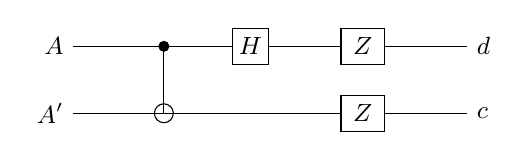
\begin{tikzpicture}[x=1cm,y=1cm,>=Stealth,font=\small]
\draw (0,0)--(5,0);\draw (0,-.85)--(5,-.85);
\node[left] at(0,0){$A$};\node[left] at(0,-.85){$A'$};
\fill (1.15,0) circle(2pt);\draw (1.15,0)--(1.15,-.85);
\draw (1.15,-.85) circle(.12);\draw (1.03,-.85)--(1.27,-.85);
\draw[fill=white] (2.02,-.23)rectangle(2.48,.23);\node at(2.25,0){$H$};
\foreach \y in {0,-.85}{\draw[fill=white](3.4,\y-.23)rectangle(3.95,\y+.23);\node at(3.675,\y){$Z$};}
\node[right]at(5,0){$d$};\node[right]at(5,-.85){$c$};
\end{tikzpicture}
\caption{The running qubit example. A controlled-NOT followed by a Hadamard gate and computational readout measures the aligned Bell labels: $c$ is the $Z\otimes Z$ parity and $d$ the $X\otimes X$ parity. Four orthogonal Bell states fill the four-dimensional space, so no residual label remains. A Hadamard on the second input converts this to the crossed context.}
\label{fig:decoder}
\end{figure}

For the running qubit example, the four Bell states constitute a saturating frame. The parity readout in Fig.~\ref{fig:decoder} has no residual record, even with a correlated finite-dimensional quantum spectator. A Hadamard gate interchanges the tested $Z$ and $X$ attributes and produces the crossed context. Appendix~\ref{app:quantum} verifies the capacity and circuit claims directly.

\subsection{What no-hypersignaling would supply}
The capacity premise concerns the size of a perfectly readable alphabet. No-hypersignaling concerns a different quantity: the classical cost of reproducing every finite prepare-and-read channel, with shared randomness allowed \cite[Definitions 2--3, Eq.~(2)]{hs}. The connection is useful, but it requires stating which attributes can be prepared.

In this subsection, assume that each nonempty attribute in a finite discrimination frame contains an available complete preparation. In particular, this applies to a proposed residual attribute. This preparation-access premise extends VI, whose wording guarantees preparation of information-instantiating attributes \cite[Sec.~6, VI, p.~13]{cti}. It is an explicit premise when applied to arbitrary residual attributes, not a consequence of their being nonempty.

Write $s(S)$ for the signaling dimension, with value infinity if no finite simulator exists. It is the smallest integer $m$ such that every finite channel $p(j\mid i)$ obtained by preparing $S$ and making one fixed readout can be simulated by sending one of $m$ classical symbols, with free shared randomness. There is no independently chosen input at the receiver. Equivalently, each such channel belongs to the convex hull of deterministic maps whose image has at most $m$ elements. The classical simulator is only a benchmark; no hidden stochastic dynamics is assumed for $S$.

Any $m$-symbol channel with the same $N$ input and output labels satisfies
\begin{equation}\label{eq:diagonal}
 \sum_{i=1}^N p(i\mid i)\leq m.
\end{equation}
Indeed, a deterministic map with at most $m$ output values has at most $m$ fixed points. Convex mixtures preserve the inequality. An $N$-label discriminator with worst-case preparation-and-readout error at most $\xi$ gives the opposite bound $N(1-\xi)$ on this sum. Letting $\xi$ vanish proves
\begin{equation}\label{eq:caps}
 \capn(S)\leq s(S)
\end{equation}
under preparation access. The closed classical polytope includes the ideal task limit.

\begin{corollary}[A no-hypersignaling certificate for parity coverage]\label{cor:hs}
Assume the hypotheses of Theorem~\ref{thm:capacity} and preparation access for its frames. Let $\capn(R)=n$. Suppose the local prepare-and-read simulations obey
\begin{equation}\label{eq:localbudgets}
 s(S_A)=2,\qquad s(R)=n,
\end{equation}
and no-hypersignaling holds on the relevant composite:
\begin{equation}\label{eq:nohs}
 s(S_A\otimes S_A\otimes R)\leq s(S_A)^2s(R).
\end{equation}
Then the aligned parity domain is exhaustive. The reversible setting interchange of Eq.~\eqref{eq:interchange} makes the crossed domain exhaustive too. With H, C, the finite-record bridge, and independent-copy factorization as in Theorem~\ref{thm:bell}, the consequence is $|B|\leq2\sqrt2$.

More explicitly, a missing aligned domain with a preparable residual would permit a channel on $N=4n+1$ labels for which
\begin{equation}\label{eq:witness}
\begin{aligned}
 \frac1{4n+1}\sum_i p(i\mid i)&\geq1-\xi,\\
 \frac1{4n+1}\sum_i p(i\mid i)&\leq\frac{4n}{4n+1}\quad\text{(classical)}.
\end{aligned}
\end{equation}
The second line applies to every $4n$-symbol simulator. Thus any realization with $\xi<1/(4n+1)$ violates that simulation bound.
\end{corollary}
\begin{proof}
Equations~\eqref{eq:caps}--\eqref{eq:nohs} imply Eq.~\eqref{eq:capacity}; Theorem~\ref{thm:capacity} then applies. Alternatively, its construction supplies $4n$ calibration labels and one residual label. Preparation access and IV turn them into a nearly noiseless $4n+1$-label channel. Equation~\eqref{eq:diagonal} proves Eq.~\eqref{eq:witness}, contradicting Eq.~\eqref{eq:nohs} at sufficiently small $\xi$.
\end{proof}

This is the distinguishable-message instance of the communication-game witness used to formulate no-hypersignaling \cite[Eq.~(3)]{hs}. The task result supplies its messages from a failed parity domain. Without Eq.~\eqref{eq:localbudgets}, no-hypersignaling gives only $\capn(S_A^{\otimes2}R)\leq s(S_A)^2s(R)$, not the required $4n$. It is therefore stronger than the capacity upper bound only after these local simulation budgets and preparation access are fixed.

The distinction is strict in general operational theories. For the elementary square and product-state composite in the hypersignaling model of Ref.~\cite{hs}, the largest jointly readable alphabets have sizes two and four. Nevertheless, a seven-preparation channel defeats every four-symbol simulation by the exact payoff gap $1/2-10/21=1/42$. Appendix~\ref{app:hs} proves the alphabet counts and checks that published witness. The square violates principle IV, so this comparison separates two capacity notions; it is not a countermodel to the constructor premises.

\section{Two finite tests of the premises}
The running qubit example isolates preparation homogeneity. A five-event certificate then excludes the joint application of H and C to specified Bell weights, without assuming any state-space geometry.

Return to
\begin{equation}\label{eq:Zplus}
 Z_+=\{\rho_A\otimes\ket+\bra+ :\rho_A\text{ arbitrary}\}.
\end{equation}
This is a closed support attribute. Together with $Z_-$ it has a unitarily readable and copyable sign label. For the total computational-bit observable $N_A+N_B$, where $N=\ket1\bra1$, its frequency vector is
\begin{equation}\label{eq:zfreq}
 \left(\frac r2,\frac12,\frac{1-r}2\right),\qquad r=\bra0\rho_A\ket0.
\end{equation}
No state in $Z_+$ lies in a sum eigenspace, and no sum eigenspace is orthogonal to all of $Z_+$. These are the relevant generalized-mixture conditions \cite[Sec.~3, ``Generalised mixtures'', pp.~17--18]{ctp}. Yet the members of $Z_+$ have different frequency partitions.

Let $F_{0,L}$ be the frequency operator for outcome zero on $L$ copies. The exact optimized error about a single common label is
\begin{equation}\label{eq:obstructionT1}
 \begin{aligned}
 &\inf_f\sup_{\rho_1,\ldots,\rho_L\in Z_+}
 \Tr\!\left[\left(\bigotimes_j\rho_j\right)(F_{0,L}-fI)^2\right]\\
 &\hspace{34mm}=\left(\frac{L+1}{4L}\right)^2.
 \end{aligned}
\end{equation}
It approaches $1/16$. For one completely specified member, the mean-square error about its own frequency is instead at most $1/(4L)$. Appendix~\ref{app:frequency} proves both statements. H therefore uses complete preparation instructions, not every copyable information label.

For a second, geometry-independent test, consider the positive nonsignalling weights
\begin{equation}\label{eq:noisybox}
 w(a,b\mid x,y)=\frac{1+(-1)^{a+b+xy}t}{4},\qquad t=\frac{81}{100}.
\end{equation}
They give $B=81/25$. The following five two-copy events, in party order $(A,B,A',B')$, are pairwise locally exclusive:
\begin{equation}\label{eq:five}
\begin{gathered}
 (0000\mid0000),\ (0011\mid0100),\ (0111\mid1101),\\
 (1100\mid1010),\ (1110\mid0011).
\end{gathered}
\end{equation}
Each wins both CHSH games. Their exact total weight is
\begin{equation}\label{eq:fiveexcess}
 5\left(\frac{181}{400}\right)^2=1+\frac{761}{32000}.
\end{equation}
This is an application of local orthogonality \cite{lo}. Under C and the discrimination principles, Theorem~\ref{thm:frequency} forces some binary comparison to differ by at least $761/160000$. Its proposed homogeneous frequency limit then obeys
\begin{equation}\label{eq:fiveH}
 \delta_{X,L}\geq\frac{761}{320000}-h\qquad\text{for every }L.
\end{equation}
Thus no theory with these covered weights can satisfy H, regardless of its geometry. The residual Bell theorem gives the additional necessary relation
\begin{equation}\label{eq:noisyresidual}
 \eps_0+\eps_1+72\kappa\geq\frac{1561}{2500}.
\end{equation}
Equation~\eqref{eq:noisyresidual} is a necessary certificate, not an assertion that these weights are compatible with H and C.

\section{Discussion}
A possible discriminator, an exhaustive measurement domain, and implementation-independent weights are distinct requirements. The information principles construct discriminators. H compares their weights, while the residual record measures the remaining domain issue. Under H, the result is $B^2\leq8+4(\eps_0+\eps_1)$. Theorem~\ref{thm:capacity} converts failure of a full domain into a surplus distinguishable label; Corollary~\ref{cor:hs} turns a preparable surplus into a communication witness.

\paragraph{States versus measurements.}
Short and Barrett show that maximal nonsignalling state spaces have no entangled effects. For one and two elementary systems their measurements are mixtures of basic sequential measurements, whereas this stronger description already fails for three systems \cite[Sec.~IV, Corollary 1, Theorems 2--4]{short}. Their result is an antecedent of the mechanism here: admitting more states can prevent a useful joint measurement. Our addition is narrower. Principles IV and V already supply a discriminator for the calibrated parity sectors, so the unresolved point becomes the domain on which that discriminator can function as the required joint measurement.

Czekaj, Horodecki, and Tylec start from three locally complete binary measurements and add a four-outcome Bell measurement with quantum-inherited parity identities. Positivity on products gives the local Bloch-ball constraint and hence quantum bipartite correlations \cite[Secs.~II--III, Eqs.~(4), (9)]{czekaj}. This is a stronger correlation conclusion under a different measurement and state-description premise. We assume neither those three coordinates nor local tomography, and do not reconstruct a ball. We retain a possible extra record and derive only the CHSH consequence supported by its weight. Their noisy Bell effects also differ from our residual record, which is a calibrated outcome, not an unsharpness parameter.

Selby and collaborators study parity-reading effects through compositional positivity constraints \cite[Secs.~3, 5, 7--8]{selby}. Their Sec.~7.1 already recovers the CHSH quantum bound numerically in specified locally tomographic two- and three-fiducial-measurement cases. Our contribution is not that parity readout can restrict CHSH. It is an analytic implication from the stated task and calibration premises, with an explicit residual-domain term. Their general parity-reading conjecture remains distinct from this conditional result. Restricted-effect models likewise motivate keeping the available transformations explicit \cite{restricted}; the present theorems do not infer the availability of every positive functional.

\paragraph{Exclusivity and sharpness.}
Cabello's extra two-copy contexts are the direct antecedent of P \cite[step III and Eq.~(10)]{cabello}. Our sixteen-set generator certifies his counting construction for arbitrary biased weights. The new quantitative term is the retained residual weight, not a new route from exclusivity alone to Tsirelson's bound. Chiribella and Yuan instead obtain exclusivity from repeatability, minimal disturbance, and closure of sharp measurements \cite[Principles 1--3 and Methods]{sharp}. Our frequency-neutral completion bypasses that instrument-level assumption. The reset example in Appendix~\ref{app:quantum} shows why retaining an input attribute is weaker than minimal disturbance.

The finite-copy LO conclusion uses the principle of Fritz and collaborators \cite{lo}. It is not identified with the almost-quantum representation of Navascu\'es and collaborators \cite[Definition 1]{aq}, whose vector structure already bounds CHSH. Nor is the present proof an uncertainty-and-steering derivation of the kind given by Oppenheim and Wehner \cite{uncertainty}. These distinctions delimit the contribution: it is a task formulation with a finite-resolution estimate and a residual-domain certificate, not a quantum reconstruction.

\paragraph{Capacity and the remaining implication.}
The source's classical-capacity additivity statement and Hardy's capacity composition rule precede the sufficient bound used here \cite[Sec.~4, p.~10]{cti}\cite[Axiom 4]{hardy}. Section~5.2 explains the preparation-access condition that connects the source's information variables to the frames counted in Theorem~\ref{thm:capacity}. Dall'Arno and collaborators constrain the larger signaling-simulation problem \cite[Definitions 2--3]{hs}. Our no-hypersignaling corollary needs both access to the residual preparations and the stated local simulation budgets; under those conditions a missing domain has the communication test in Eq.~\eqref{eq:witness}.

H, C, the finite-record rules, and independent-copy factorization are added premises. T2 yields the aligned sectors, not the global binary capacity in Eq.~\eqref{eq:capacity}; the qutrit embedding already separates those assertions. We have not derived the reversible setting interchange, or preparation-specific coverage P, from T2 and the information principles. Nor have we constructed a superquantum theory satisfying all those source premises. The remaining Bell question concerns coverage of the tested preparation, not the already-false unrestricted inference from a binary sector to global binary capacity.

For a universal Bell bound, the selected T2 settings must also cover the tested settings or experiments approaching the theory's supremum. Requiring P for every setting pair would be too strong: the tilted-qubit example in Appendix~\ref{app:quantum} lacks an exhaustive aligned domain. Failure of one sufficient certificate does not establish independence of P.

\paragraph{Reproducibility.}
The source package contains this manuscript, its TikZ and pgfplots figures, a build script, and exact certificate code. The code checks the finite enumeration, rational identities, and quantum examples; it is not a formalization of the universal task theorems.

\begin{thebibliography}{20}
\raggedright
\bibitem{DM}
David Deutsch and Chiara Marletto.
\newblock Constructor theory of information.
\newblock \href{https://doi.org/10.1098/rspa.2014.0540}{\emph{Proceedings of the Royal Society A} \textbf{471}, 20140540 (2015)}.
\newblock \href{https://arxiv.org/abs/1405.5563v2}{arXiv:1405.5563v2}.

\bibitem{M}
Chiara Marletto.
\newblock Constructor theory of probability.
\newblock \href{https://doi.org/10.1098/rspa.2015.0883}{\emph{Proceedings of the Royal Society A} \textbf{472}, 20150883 (2016)}.
\newblock \href{https://arxiv.org/abs/1507.03287v3}{arXiv:1507.03287v3}.

\bibitem{OW}
Jonathan Oppenheim and Stephanie Wehner.
\newblock The uncertainty principle determines the non-locality of quantum mechanics.
\newblock \href{https://doi.org/10.1126/science.1192065}{\emph{Science} \textbf{330}, 1072--1074 (2010)}.
\newblock \href{https://arxiv.org/abs/1004.2507v2}{arXiv:1004.2507v2}.

\bibitem{CY}
Giulio Chiribella and Xiao Yuan.
\newblock Measurement sharpness cuts nonlocality and contextuality in every physical theory.
\newblock \href{https://arxiv.org/abs/1404.3348v2}{arXiv:1404.3348v2 (2014)}.

\bibitem{Cabello}
Ad\'an Cabello.
\newblock Exclusivity principle and the quantum bound of the Bell inequality.
\newblock \href{https://doi.org/10.1103/PhysRevA.90.062125}{\emph{Physical Review A} \textbf{90}, 062125 (2014)}.
\newblock \href{https://arxiv.org/abs/1406.5656v3}{arXiv:1406.5656v3}.

\bibitem{JL}
Peter Janotta and Raymond Lal.
\newblock Generalized probabilistic theories without the no-restriction hypothesis.
\newblock \href{https://doi.org/10.1103/PhysRevA.87.052131}{\emph{Physical Review A} \textbf{87}, 052131 (2013)}.
\newblock \href{https://arxiv.org/abs/1302.2632v1}{arXiv:1302.2632v1}.

\bibitem{KL}
Emanuel Knill and Raymond Laflamme.
\newblock Theory of quantum error-correcting codes.
\newblock \href{https://doi.org/10.1103/PhysRevA.55.900}{\emph{Physical Review A} \textbf{55}, 900--911 (1997)}.
\newblock \href{https://arxiv.org/abs/quant-ph/9604034}{arXiv:quant-ph/9604034}.

\bibitem{Fritz}
Tobias Fritz, Ana Bel\'en Sainz, Remigiusz Augusiak, Jonatan Bohr Brask, Rafael Chaves, Anthony Leverrier, and Antonio Ac\'in.
\newblock Local orthogonality as a multipartite principle for quantum correlations.
\newblock \href{https://doi.org/10.1038/ncomms3263}{\emph{Nature Communications} \textbf{4}, 2263 (2013)}.
\newblock \href{https://arxiv.org/abs/1210.3018v3}{arXiv:1210.3018v3}.

\bibitem{AQ}
Miguel Navascu\'es, Yelena Guryanova, Matty J. Hoban, and Antonio Ac\'in.
\newblock Almost quantum correlations.
\newblock \href{https://doi.org/10.1038/ncomms7288}{\emph{Nature Communications} \textbf{6}, 6288 (2015)}.
\newblock \href{https://arxiv.org/abs/1403.4621v1}{arXiv:1403.4621v1}.

\bibitem{Selby}
John H. Selby, Ana Bel\'en Sainz, Victor Magron, \L ukasz Czekaj, and Micha\l{} Horodecki.
\newblock Correlations constrained by composite measurements.
\newblock \href{https://doi.org/10.22331/q-2023-08-10-1080}{\emph{Quantum} \textbf{7}, 1080 (2023)}.
\newblock \href{https://arxiv.org/abs/2009.04994v4}{arXiv:2009.04994v4}.

\bibitem{Hardy}
Lucien Hardy.
\newblock Quantum theory from five reasonable axioms.
\newblock \href{https://arxiv.org/abs/quant-ph/0101012v4}{arXiv:quant-ph/0101012v4 (2001)}.


\bibitem{SB}
Anthony J. Short and Jonathan Barrett.
\newblock Strong nonlocality: A trade-off between states and measurements.
\newblock \href{https://doi.org/10.1088/1367-2630/12/3/033034}{\emph{New Journal of Physics} \textbf{12}, 033034 (2010)}.
\newblock \href{https://arxiv.org/abs/0909.2601v2}{arXiv:0909.2601v2}.

\bibitem{CHT}
\L ukasz Czekaj, Micha\l{} Horodecki, and Tomasz Tylec.
\newblock Bell measurement rules out supraquantum correlations.
\newblock \href{https://doi.org/10.1103/PhysRevA.98.032117}{\emph{Physical Review A} \textbf{98}, 032117 (2018)}.
\newblock \href{https://arxiv.org/abs/1802.09510v2}{arXiv:1802.09510v2}.

\bibitem{NHS}
Michele Dall'Arno, Sarah Brandsen, Alessandro Tosini, Francesco Buscemi, and Vlatko Vedral.
\newblock No-hypersignaling principle.
\newblock \href{https://doi.org/10.1103/PhysRevLett.119.020401}{\emph{Physical Review Letters} \textbf{119}, 020401 (2017)}.
\newblock \href{https://arxiv.org/abs/1609.09237v3}{arXiv:1609.09237v3}.

\end{thebibliography}



\appendix
\section{Task closure and the completion argument}\label{app:closure}
The proofs use ideal calibration tasks and their limiting readout weights, as specified in Sec.~2. Empty outcomes are omitted; a constant detector handles the associated trivial variables \cite[Sec.~6, footnote on p.~15]{cti}.

\subsection{Orthogonality closure}
Principle V and symmetry imply
\begin{equation}\label{eq:statewise}
 a\perp b\quad\Longleftrightarrow\quad
 \forall s\in a,\ t\in b:\ \{s\}\perp\{t\}.
\end{equation}
For the reverse direction, first use V to infer $\{s\}\perp b$ for each $s$, then use it again for $a$. Hence the bar operation is the polarity of a symmetric, irreflexive relation on states. It reverses inclusions, $a\subseteq\ddbar a$, and $\overline{\ddbar a}=\overline a$. Double bar is therefore extensive, monotone, and idempotent. Its closed sets are closed under intersections. Moreover,
\begin{equation}\label{eq:polarity}
 \overline{a\cup b}=\overline a\cap\overline b,
 \qquad \overline a\cap\cl(a)=\varnothing.
\end{equation}
The second equality follows because a state in the intersection would be orthogonal to itself. These facts prove the closure claims used in Eq.~\eqref{eq:completion}.

\subsection{Calibration on the closure of an attribute}
For any attribute $a$, the pair $\{\cl(a),\overline a\}$ is distinguishable by IV and V and has full domain. A measurer of it also measures $\{a,\overline a\}$. If a variable $X$ contains $a$, the Boolean measurer is a measurer of the binary coarse-graining that asks whether the input label is $a$. By VIII, all measurers of that coarse-graining are sharp on $\cl(a)$, since $\cl(a)\subseteq D_X$. This proves the closure property used for frequency windows and parity sectors.

A Boolean measurer can have sharp yes only on its closed yes attribute. Indeed, on a sharp-yes input $s$, that same measurer distinguishes $\{s\}$ from the no attribute $\overline a$. Thus $s\in\cl(a)$. Conversely, sharp yes on $\cl(a)$ is its calibration. No inference from the numerical condition $w=1$ to sharpness is involved.

\subsection{Full completion and comparison with the original contexts}
Let $x_i$ be the finite family of nonempty closed, pairwise distinguishable attributes in Theorem~\ref{thm:frequency}, and $r=\overline{\bigcup_i x_i}$. By Eq.~\eqref{eq:polarity}, the closure of their union with $r$ is $\Omega$. All members are distinguishable, including $r$ when nonempty. Let $D$ be the common discriminator from IV.

For fixed $i$, put $b_i=r\cup\bigcup_{j\ne i}x_j$. The coarse-graining $D_i$ is calibrated on $Y_i=\{x_i,b_i\}$, and $D_{Y_i}=\Omega$. Since $b_i\subseteq\overline{x_i}$, a Boolean measurer $T_i$ of $\{x_i,\overline{x_i}\}$ is also a measurer of $Y_i$. It is sharp no on $\overline{x_i}$. VIII, applied on $D_{Y_i}$, forces $D_i$ to be sharp no there too. It is already sharp yes on $x_i$. Thus $D_i$ is a Boolean measurer on all of $\Omega$.

Now let the original event arise as outcome $x_i$ of context $X_i$. Both $D_i$ and the original coarse detector measure
\begin{equation}\label{eq:comparison-variable}
 V_i=\left\{x_i,\ \bigcup_{x\in X_i,\ x\ne x_i}x\right\},
\end{equation}
whose domain equals $D_{X_i}$. Coverage puts the tested preparation in that domain. Equation~\eqref{eq:neutral} then compares the original event weight with the corresponding $D$ outcome. If a covered event is a coarse union rather than a closed outcome, replace that union by its closure; the preceding calibration property makes the replacement a closed event with the same detector on its legitimate domain.

When $\Delta>0$ in Eq.~\eqref{eq:converse}, $\sum_i w(D,i\mid\omega)\leq1$ gives
\begin{equation}\label{eq:excess-sum}
 \sum_i\bigl[w(e_i\mid\omega)-w(D,i\mid\omega)\bigr]\geq\Delta.
\end{equation}
At least one summand is at least $\Delta/m$. Combining it with Eq.~\eqref{eq:neutral} proves the stated lower bound for every $L$ and $f$.

\subsection{Approximation and task possibility}
For each $L$, the completion uses only finitely many discriminators, relabellings, and parallel networks. Under the task-accuracy convention, successively more accurate realizations retain all terminal records, including failure records, while uniform calibration errors vanish. Equations~\eqref{eq:mean}, \eqref{eq:ce}, and \eqref{eq:sum16} are finite inequalities in bounded record weights and persist in that limit. The frequency limit $L\to\infty$ is taken after fixing the finite-resolution task and its ideal readout weights; no unbounded constructor is claimed to be a finite apparatus.

\section{Frequency homogeneity and its quantum consistency}\label{app:frequency}
\subsection{A uniform partition is a homogeneous attribute}
Let $P_1,\ldots,P_k$ be a projective observable in finite dimension and let $A$ be an attribute of density operators. Define
\begin{equation}\label{eq:frequency-operator}
 F_{j,L}=\frac1L\sum_{\ell=1}^L P_j^{(\ell)}.
\end{equation}
A common frequency vector $f$ in mean square on all independent products from $A$ exists if and only if
\begin{equation}\label{eq:constant-frequencies}
 \Tr(\rho P_j)=f_j\quad\text{for every }\rho\in A\text{ and every }j.
\end{equation}
To prove this, set $p_{j,\ell}=\Tr(\rho_\ell P_j)$ and $\overline p_j=L^{-1}\sum_\ell p_{j,\ell}$. Direct expansion gives
\begin{equation}\label{eq:variance}
\begin{aligned}
 &\Tr\!\left[\left(\bigotimes_{\ell=1}^L\rho_\ell\right)(F_{j,L}-f_j I)^2\right]\\
 &\hspace{4mm}=(\overline p_j-f_j)^2+
 \frac1{L^2}\sum_{\ell=1}^L p_{j,\ell}(1-p_{j,\ell}).
\end{aligned}
\end{equation}
Taking every factor equal proves necessity. If Eq.~\eqref{eq:constant-frequencies} holds, the right side is at most $1/(4L)$ for every product, which proves sufficiency. For a closed support attribute consisting of all density operators on a subspace $S$, this is equivalent to
\begin{equation}\label{eq:compression}
 P_S P_j P_S=f_jP_S.
\end{equation}
The equivalence follows by evaluating all pure-state quadratic forms on $S$ and using polarization. This scalar-compression calculation is elementary; the analogous structure for a general error family appears in quantum error correction \cite{qec}.

\subsection{The exact one-sixteenth obstruction}
For $Z_+$, the probability or frequency parameter of outcome zero is $p\in[0,1/2]$. The quantum frequency identification here is the one explicitly made in Ref.~\cite[Sec.~5, E2, p.~28]{ctp}. For fixed mean $q=L^{-1}\sum_\ell p_\ell$, concavity of $p(1-p)$ bounds Eq.~\eqref{eq:variance} by
\begin{equation}\label{eq:qbound}
 (q-f)^2+\frac{q(1-q)}L,
\end{equation}
with equality when all $p_\ell=q$. This expression is convex in $q\in[0,1/2]$, including the affine case $L=1$. Its maximum is therefore
\begin{equation}\label{eq:endpointmax}
 \max\left\{f^2,\ (1/2-f)^2+\frac1{4L}\right\}.
\end{equation}
The minimum occurs when the two entries agree, at $f=(L+1)/(4L)$, proving Eq.~\eqref{eq:obstructionT1}.

The sign attributes $Z_\pm$ are closed because they are complete density-operator attributes on orthogonal subspaces. Applying $Z$ to the second qubit exchanges the signs. A controlled sign flip on a blank target copies the label; equivalently, conjugate a controlled-NOT by Hadamard gates on its source and target sign qubits. The unknown first qubit is untouched. Neither of the subspaces $\mathbb C^2\otimes\Span\{\ket\pm\}$ has a nonzero intersection with any eigenspace of $N_A+N_B$, but each has nonzero overlap with each eigenspace. This proves the generalized-mixture and information-variable assertions used in Sec.~6.

\begin{figure}[!htbp]
\centering
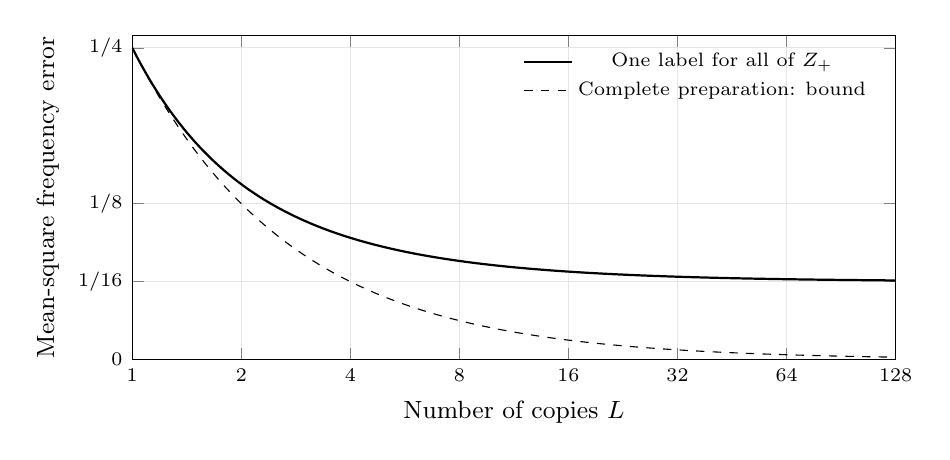
\begin{tikzpicture}
\begin{axis}[width=.93\columnwidth,height=5.7cm,
 xmode=log,log basis x=2,xmin=1,xmax=128,ymin=0,ymax=.26,
 xtick={1,2,4,8,16,32,64,128},xticklabels={1,2,4,8,16,32,64,128},
 ytick={0,.0625,.125,.25},yticklabels={$0$,$1/16$,$1/8$,$1/4$},
 xlabel={Number of copies $L$},ylabel={Mean-square frequency error},
 tick label style={font=\scriptsize},label style={font=\small},
 legend style={font=\scriptsize,at={(.98,.98)},anchor=north east,draw=none,fill=none},
 grid=major,grid style={gray!20}]
 \addplot[black,thick,domain=1:128,samples=180] {((x+1)/(4*x))^2};
 \addlegendentry{One label for all of $Z_+$}
 \addplot[black,dashed,domain=1:128,samples=180] {1/(4*x)};
 \addlegendentry{Complete preparation: bound}
\end{axis}
\end{tikzpicture}
\caption{A common frequency center for the unspecified first qubit leaves the exact error $((L+1)/(4L))^2$, approaching $1/16$. For one specified preparation, the variance about its own frequency is at most $1/(4L)$.}
\label{fig:frequency}
\end{figure}

\subsection{Complete quantum preparations satisfy H}
For a binary projective observable $\{P_0,P_1\}$, let $f=\Tr(\rho P_1)$ and let $Q$ be the spectral projector of $L^{-1}\sum_jP_1^{(j)}$ onto the window $[f-h,f+h]$. The input attribute in Eq.~\eqref{eq:window} is exactly the density operators supported on $Q$. From Eq.~\eqref{eq:variance} and the spectral inequality outside the window,
\begin{equation}\label{eq:quantum-tail}
 1-\Tr(Q\rho^{\otimes L})\leq\frac1{4Lh^2}.
\end{equation}
When $p=\Tr(Q\rho^{\otimes L})>0$, choose
\begin{equation}\label{eq:projected-state}
 \sigma=Q\rho^{\otimes L}Q/p.
\end{equation}
Purify $\rho^{\otimes L}$ to $\ket\psi$. Its normalized projection $\ket\phi=(Q\otimes I)\ket\psi/\sqrt p$ has squared overlap $p$. Diagonalizing the difference of their rank-one projectors in their two-dimensional span gives trace distance $\sqrt{1-p}$. Trace distance cannot increase under partial trace: in its variational expression as a supremum over effects, every effect on the reduced system is also an effect on the purification. Hence
\begin{equation}\label{eq:gentle}
 \frac12\|\rho^{\otimes L}-\sigma\|_1\leq\sqrt{1-p}.
\end{equation}
The quantum version of Eq.~\eqref{eq:metric} is bounded by trace distance, including finite ancillary readouts, again by the effect variational expression. Combining with Eq.~\eqref{eq:quantum-tail} proves Eq.~\eqref{eq:qH}; the bound one covers the remaining cases.

\section{The sixteen-set and five-set certificates}\label{app:certificates}
\subsection{Pairwise exclusivity and exact coverage}
Fix $t,c,d,k$ in Eq.~\eqref{eq:generator}, and write $k'=k\oplus1\oplus c\oplus d$. The eight fine events have Bob parity
\begin{equation}\label{eq:bob-parity}
 b\oplus b'=1\oplus\gamma_x\oplus xk\oplus(x\oplus t)k'.
\end{equation}
Its change between $x=0$ and $x=1$ is
\begin{equation}\label{eq:parity-change}
 c\oplus d\oplus k\oplus k'=1.
\end{equation}
Bob's two local settings are the same in both blocks. Two events from different blocks therefore disagree in at least one Bob output at the same setting. Events within a block differ in $a$ or $b$, also at the same setting. This proves all twenty-eight fine-event comparisons in each set. The remaining eight comparisons are supplied by the Alice parity opposite to $h_t^{cd}$. If that sector is empty, omit it and retain the same upper bound for at most nine events.

The last equation in Eq.~\eqref{eq:generator} gives
\begin{equation}\label{eq:same-status}
 a\oplus b\oplus xy=a'\oplus b'\oplus x'y'.
\end{equation}
Thus both component events win, or both lose. Conversely, consider any ordered pair satisfying Eq.~\eqref{eq:same-status}. Recover $t=x\oplus x'$, $k=y$, and $\gamma_x=1\oplus a\oplus a'$. The equation $c\oplus d=1\oplus y\oplus y'$ uniquely fixes the other $\gamma$ component. Equation~\eqref{eq:same-status} then fixes the displayed value of $b'$. The event pair occurs in exactly one generated set.

There are eight winning events and eight losing events in a single CHSH experiment. The sixteen sets therefore cover all $8^2+8^2=128$ ordered same-status pairs exactly once. Each parity outcome is included once for each $k$, hence twice. This proves Eq.~\eqref{eq:sum16} for arbitrary, possibly biased, Bell weights and certifies the construction underlying Ref.~\cite[Eq.~(10)]{cabello}.

\subsection{The residual polynomial}
Write $e=\eps_0+\eps_1$. The left side of Eq.~\eqref{eq:sum16} minus its right side is exactly
\begin{equation}\label{eq:residual-polynomial}
\begin{aligned}
 &\left(2+\frac B2\right)^2+\left(2-\frac B2\right)^2+4-2e\\
 &\quad-16-144\kappa=\frac{B^2-8-4e-288\kappa}{2}.
\end{aligned}
\end{equation}
For each $t$, the four displayed parity weights sum to $1-\eps_t$ by normalization of $\widehat J_t$, including the case of empty sectors. The eight parity weights occur twice in the sixteen event sums. This proves the residual coefficient four. The bound can also be combined with the algebraic inequality $|B|\leq4$, which follows from $|E_{xy}|\leq1$.

\subsection{The noisy-box rational certificates}
For Eq.~\eqref{eq:noisybox}, each winning event has weight $181/400$ and each losing event $19/400$. Direct summation gives normalized weights, uniform marginals independent of the remote setting, and
\begin{equation}\label{eq:box-values}
 B=\frac{81}{25},\qquad B^2-8=\frac{1561}{625}.
\end{equation}
For the five events of Eq.~\eqref{eq:five}, list their ten pairs in lexicographic order. A party witnessing equal setting and opposite output in each pair is respectively
\begin{equation}\label{eq:five-witnesses}
 3,\ 3,\ 2,\ 1,\ 2,\ 4,\ 1,\ 1,\ 4,\ 3.
\end{equation}
Each event wins both games. Equation~\eqref{eq:fiveexcess} follows by squaring its single-game weight and adding five times. Equations~\eqref{eq:converse} and \eqref{eq:kappabell} then give, without numerical approximation,
\begin{equation}\label{eq:kappa-thresholds}
 \kappa\geq\frac{761}{160000}
 \quad\text{or, with P,}\quad
 \kappa\geq\frac{1561}{180000}.
\end{equation}
The first inequality concerns the five-event completion; the second concerns the sixteen completions with P. Retaining the residual records instead gives Eq.~\eqref{eq:noisyresidual} from $B^2-8=1561/625$.

\section{Transporting closure and the T2 parity sectors}\label{app:transport}
The following lemma avoids assuming a reversible symmetry on the whole state space.

\begin{lemma}[Closure transport]\label{lem:transport}
Let $T$ be an available total transformation, including a fixed independent resource, and suppose $T(a)\subseteq b$. Then
\begin{equation}\label{eq:transport}
 T(\cl(a))\subseteq\cl(b).
\end{equation}
\end{lemma}
\begin{proof}
Follow $T$ by a Boolean measurer of $\{\cl(b),\overline b\}$. This circuit is sharp yes on $a$, so it is a measurer of the one-label calibration variable $\{a\}$. A constant-yes circuit measures the same variable and is sharp on $\cl(a)$. VIII therefore makes the composed circuit sharp yes throughout $\cl(a)$. A Boolean measurer has sharp yes only on $\cl(b)$, by Appendix~\ref{app:closure}. This proves Eq.~\eqref{eq:transport}. The one-label case uses the trivial constant-task convention.
\end{proof}

For the selected T2 sector, let $U_X^0=(x_0,x_0)\cup(x_1,x_1)$ and $U_X^1=(x_0,x_1)\cup(x_1,x_0)$; define $U_Y^0,U_Y^1$ analogously. R4 gives
\begin{equation}\label{eq:R4}
 q\subseteq\cl(U_X^0)\cap\cl(U_Y^0).
\end{equation}
The R2 task $T_X$ on the first copy maps each $U_X$ parity attribute into the opposite one while preserving both $U_Y$ parity labels. Similarly $T_Y$ exchanges the $Y$ parity and preserves the $X$ parity. These are simultaneous calibration requirements on the same implementations, as specified by R2. Lemma~\ref{lem:transport} extends these actions to the closed parity sectors.

It follows that $q,T_Xq,T_Yq,T_XT_Yq$ lie in the four sectors of Eq.~\eqref{eq:four}. Images of a nonempty physical attribute under a total available transformation are nonempty. Any two of these four attributes differ in an $X$ or $Y$ parity, and the corresponding parity measurer distinguishes them. Their enclosing intersections of closed sectors are also pairwise distinguishable and closed. IV supplies a common four-valued discriminator.

\subsection{Reversible transport and spectator-stable saturation}
If $G$ and $G^{-1}$ are available total transformations, applying Lemma~\ref{lem:transport} in both directions gives
\begin{equation}\label{eq:reversible-closure}
 G(\cl(a))=\cl(G(a)).
\end{equation}
The same maps preserve distinguishability: a discriminator can be preceded by the inverse transformation. Hence $G(\overline a)=\overline{G(a)}$. In particular, Eq.~\eqref{eq:interchange} on the second Alice copy maps the aligned product calibration unions to the crossed unions. Equation~\eqref{eq:reversible-closure} then maps each closed parity sector, its intersections, and its union closure as claimed in Theorem~\ref{thm:capacity}.

Here is the general saturation criterion. Let $K$ be an active composite with pairwise distinguishable closed attributes $h_1,\ldots,h_k$. Suppose their union contains a frame $\{f_1,\ldots,f_M\}$, each $f_i$ lying in one of the $h_j$. For a spectator $R$ with $\capn(R)=n$, assume the extended sectors contain every independent product $f_i\otimes z$, with $z$ a spectator attribute. If
\begin{equation}\label{eq:general-capacity}
 \capn(K\otimes R)\leq Mn,
\end{equation}
then the extended sectors have full domain.

To prove the claim, choose an $n$-element frame $\{z_j\}$. The $Mn$ product attributes $f_i\otimes z_j$ are pairwise distinguishable: a discriminator on $K$ separates different $i$, and one on $R$ separates different $j$. All products belong to the extended union. A nonempty bar of this union would supply a further distinguishable attribute, contradicting Eq.~\eqref{eq:general-capacity}. Its bar is therefore empty, which is exactly full double-bar coverage. If $M=\capn(K)$, the premise is the spectator-stable upper half of multiplicativity. The upper bound concerns the full composite, including correlated residual attributes, not just the independent calibration products.

\section{Quantum examples and comparisons}\label{app:quantum}
\subsection{Saturation and the parity domains}
Use $\ket\Phi=(\ket{00}+\ket{11})/\sqrt2$ in each Bell experiment. Alice measures $A_0=Z$, $A_1=X$, and Bob measures
\begin{equation}\label{eq:bob-observables}
 B_0=(Z+X)/\sqrt2,\qquad B_1=(Z-X)/\sqrt2.
\end{equation}
The correlators are $(1,1,1,-1)/\sqrt2$, obtained directly from $\langle Z\otimes Z\rangle=\langle X\otimes X\rangle=1$ and the vanishing cross correlators. Hence $B=2\sqrt2$.

On Alice's doubled subsystem the aligned parity operators are $Z\otimes Z$ and $X\otimes X$. The crossed operators are $Z\otimes X$ and $X\otimes Z$. In each pair the operators commute and square to the identity. Their four joint projectors are
\begin{equation}\label{eq:joint-projectors}
 \Pi^{cd}=\frac14(I+(-1)^cC_0)(I+(-1)^dC_1).
\end{equation}
They are orthogonal, have trace one, and sum to the identity. Thus their support attributes cover every two-qubit preparation, including arbitrary spectators. They realize P without imposing a two-coordinate local state space. The decoder in Fig.~\ref{fig:decoder} is $U=(H\otimes I)\operatorname{CNOT}$, where $H=(X+Z)/\sqrt2$. Direct conjugation gives
\begin{equation}\label{eq:decoder}
\begin{aligned}
 U^\dagger(Z\otimes I)U&=X\otimes X,\\
 U^\dagger(I\otimes Z)U&=Z\otimes Z.
\end{aligned}
\end{equation}
Also $HZH=X$ and $HXH=Z$, proving the setting-interchange property and the crossed decoder.

A quantum system of Hilbert-space dimension $D$ has information capacity $D$. Orthogonal pure states attain this value. Conversely, an effect that accepts every state of an attribute and rejects every state of another forces their support subspaces to be orthogonal. Indeed, $0\leq E\leq I$ and $\Tr(E\rho)=1$ imply that $E$ is the identity on $\supp\rho$, whereas $\Tr(E\sigma)=0$ implies it vanishes on $\supp\sigma$. Arbitrarily accurate discrimination gives the same conclusion by compactness of the effect interval. A finite frame thus occupies pairwise orthogonal nonzero subspaces, so its cardinality cannot exceed $D$. A spectator of dimension $D_R$ gives capacity $4D_R$ for Alice's doubled qubit and the spectator. This proves Eq.~\eqref{eq:capacity} for the full quantum composite, not just its product states.

The distinction between a binary sector and a binary-capacity carrier can be seen in a qutrit. Take $x_0,x_1$ to be the pure-state attributes of $\ket0,\ket1$, and $y_0,y_1$ those of $(\ket0\pm\ket1)/\sqrt2$. The selected two-attribute variables are legitimate information observables without being maximal \cite[Sec.~7, p.~19]{cti}. Extend the qubit flips and the Hadamard gate by the identity on $\ket2$. The generalized-mixture relations, simultaneous flip calibrations, intrinsic measurement attributes, and the state $\ket\Phi$ then satisfy R1--R4 within the two-level sector. The four aligned Bell sectors span only the four-dimensional space $\Span\{\ket0,\ket1\}^{\otimes2}$. Their residual support is five-dimensional and contains $\ket{22}$. Nevertheless, $\capn(S_A)=3$ and $\capn(S_A\otimes S_A)=9$. Thus T2 does not imply the full-carrier bound in Eq.~\eqref{eq:capacity}, even with a trivial spectator. Preparations covered by the selected binary local observables still lie in the two-level sector and satisfy P in this example.

\subsection{Parity coverage is not automatic for arbitrary quantum settings}
Let $A_0=Z$ and $A_1=(3Z+4X)/5$. They are binary projective observables because $A_1^2=I$. Their aligned parity operators satisfy
\begin{equation}\label{eq:tilted-commutator}
 [A_0\otimes A_0,A_1\otimes A_1]
 =\frac{24i}{25}(I\otimes Y+Y\otimes I),
\end{equation}
whose operator norm is $48/25$. The norm follows from the eigenvalues $2,0,0,-2$ of the parenthesized operator. If their common eigenspaces spanned the whole space, a basis of common eigenvectors would make the operators commute. Equation~\eqref{eq:tilted-commutator} rules that out. Thus their common parity-sector variable does not have full domain, although it can still cover particular preparations.

\subsection{Nonperturbation need not be minimal disturbance}
On two qubits, consider the instrument
\begin{equation}\label{eq:reset}
 \mathcal M_i(\rho)=\ket{i0}\bra{i0}\,
 \Tr[(\ket i\bra i\otimes I)\rho],\quad i=0,1.
\end{equation}
It is completely positive, and its sum preserves trace. It reads the first-qubit label and leaves that label unchanged, so it is nonperturbing on its calibrated attributes and repeatable. The compatible readout $Q=I\otimes\ket1\bra1$ has weight one on $\ket{01}\bra{01}$ and zero after the instrument. The disturbance is exactly one. It therefore fails the minimal-disturbance condition of Ref.~\cite[Eq.~(4)]{sharp}. The same first-qubit effects do admit a L\"uders implementation; this example separates instrument conditions, not their possible statistics.

\subsection{The almost-quantum comparison}
The representation in Ref.~\cite[Definition 1 and Sec.~6]{aq} assigns projectors to local outcomes and a state on which the relevant products have the required order independence. For binary outcomes put $A_x=P_0^x-P_1^x$ and $B_y=Q_0^y-Q_1^y$. On that state $\ket\psi$, define unit vectors $u_x=A_x\ket\psi$ and $v_y=B_y\ket\psi$. Their real inner products are the correlators. Therefore
\begin{equation}\label{eq:gram-bound}
\begin{aligned}
 |B|&\leq\|v_0+v_1\|+\|v_0-v_1\|\\
 &\leq\sqrt{2\bigl(\|v_0+v_1\|^2+\|v_0-v_1\|^2\bigr)}
 =2\sqrt2.
\end{aligned}
\end{equation}
This is the standard Gram-vector bound for that representation.

\section{Readable labels and the published hypersignaling witness}\label{app:hs}
This appendix separates two dimension notions using the HS model of Ref.~\cite[Eq.~(4) and Supplemental Material]{hs}. The model and the seven-input witness are prior work. We give an analytic proof of its readable-alphabet bound and evaluate the witness exactly.

\subsection{Two locally readable labels, four jointly}
For this comparison only, let $\drec(S)$ be the maximum number of prepared states distinguished by one measurement. Under IV and preparation access it equals $\capn(S)$, but we will not impose IV on the comparison model.

The elementary normalized state space is the convex hull of
\begin{equation}\label{eq:hs-states}
\begin{aligned}
 v_0&=(1,0,1)^T,&v_1&=(0,1,1)^T,\\
 v_2&=(-1,0,1)^T,&v_3&=(0,-1,1)^T.
\end{aligned}
\end{equation}
The unit effect is $u=(0,0,1)^T$, and all positive effects are allowed. The four extreme rays of the effect cone are
\begin{equation}\label{eq:hs-effects}
\begin{aligned}
 e_0&=(1,1,1)^T,&e_1&=(-1,1,1)^T,\\
 e_2&=(-1,-1,1)^T,&e_3&=(1,-1,1)^T.
\end{aligned}
\end{equation}
These rays follow by imposing nonnegative evaluation on the four displayed vertices. Any finite measurement can be refined into effects proportional to $e_i$. Normalization forces their total coefficients to have the form $(a,b,a,b)$ with $2a+2b=1$. Thus every measurement is a mixture of the two binary measurements $\{e_0/2,e_2/2\}$ and $\{e_1/2,e_3/2\}$, followed by classical postprocessing. Sending the binary outcome simulates any such readout with shared randomness. Hence $s(S)=2$, with equality because $v_0,v_2$ are perfectly distinguishable.

Let $c=(0,0,1)^T$ denote the center state. Since $2c-v_i$ is a normalized state, any effect $f$ satisfies $f(v_i)\leq2f(c)$, and convexity extends this to every normalized state. If $N$ states are read with error at most $\xi$, summing over their respective effects gives $N(1-\xi)\leq2$. Consequently $\drec(S)=2$.

The bipartite normalized states are all convex mixtures of $v_i\otimes v_j$, again with all positive effects. Cone positivity gives
\begin{equation}\label{eq:hs-cone}
\begin{aligned}
 4c\otimes c-v_i\otimes v_j
 &=(2c-v_i)\otimes2c\\
 &\quad+v_i\otimes(2c-v_j)\geq0.
\end{aligned}
\end{equation}
Applying the same bound to every outcome of a common measurement gives $N(1-\xi)\leq4$. The products of $v_0,v_2$ form a four-label readable frame, so
\begin{equation}\label{eq:hs-readable}
 \drec(S\otimes S)=4=\drec(S)^2.
\end{equation}
This proof includes arbitrary mixed preparations and arbitrarily accurate discrimination limits.

Each pair of different elementary vertices can nevertheless be distinguished by some binary measurement: evaluation of the $e_i/2$ gives an opposite sharp pair. Since no one measurement distinguishes all four, principle IV fails. The comparison therefore does not decide whether the two dimension notions can differ under every constructor premise.

\subsection{A channel that needs more than four classical symbols}
Represent the product state $v_i\otimes v_j$ by the matrix $\Omega_{4i+j}=v_iv_j^T$, and put $E_{4i+j}=e_ie_j^T$, with $i,j\in\{0,1,2,3\}$. Matrix evaluation is $\Tr(\Omega^TE)$. Define
\begin{equation}\label{eq:e23}
 E_{23}=\begin{pmatrix}-1&-1&0\\1&-1&0\\0&0&1\end{pmatrix}.
\end{equation}
The subscript follows the source's enumeration. The seven measurement effects are
\begin{equation}\label{eq:hs-measurement}
 \frac18 E_0,\ \frac18 E_1,\ \frac18 E_6,\ \frac18 E_8,
 \ \frac18 E_{10},\ \frac18 E_{15},\ \frac14 E_{23}.
\end{equation}
Their sum is $uu^T$. The first six terms are positive products. Since the planar parts of $v_i,v_j$ are signed coordinate vectors, $E_{23}$ evaluates to either zero or two on every product vertex. Convexity proves validity on the entire declared state space.

For preparations $(\Omega_0,\Omega_2,\Omega_6,\Omega_7,\Omega_{12},\Omega_{13},\Omega_{15})$, respectively, the two nonzero output positions in each row are
\begin{equation}\label{eq:hs-channel}
\begin{gathered}
 (1,6),\ (2,7),\ (2,3),\ (3,7),\\
 (4,6),\ (4,7),\ (5,6).
\end{gathered}
\end{equation}
Each displayed position has weight $1/2$, defining a channel $\Xi$. This is the channel in Ref.~\cite[Eq.~(4)]{hs}. Its payoff matrix is
\begin{equation}\label{eq:payoff}
 \Gamma=\frac1{21}\begin{pmatrix}
 2&0&0&0&0&1&0\\
 0&2&0&0&0&0&2\\
 0&2&2&0&0&0&0\\
 0&0&2&0&0&0&2\\
 0&0&0&1&0&1&0\\
 0&0&0&1&0&0&0\\
 0&0&0&0&2&1&0
 \end{pmatrix}.
\end{equation}
Direct substitution gives $\sum_{ij}\Gamma_{ij}\Xi_{ij}=1/2$.

A deterministic four-symbol simulation uses a set $J$ of at most four output columns, so its best payoff is $\sum_i\max_{j\in J}\Gamma_{ij}$. Nonnegative entries let us enlarge $J$ to four columns. Let $k$ count the selected columns from $\{2,3,7\}$, let $l$ count those from $\{1,4,5\}$, and let $b$ indicate whether column six is selected. Then $k+l+b=4$. The unscaled row-maximum sum is exactly
\begin{equation}\label{eq:hs-score}
\begin{gathered}
 r(k)+2l+b(3-l),\\
 (r(0),r(1),r(2),r(3))=(0,4,6,6).
\end{gathered}
\end{equation}
For $b=0$, the pair $(k,l)$ is $(1,3),(2,2)$, or $(3,1)$, giving respective scores $10,10$, and $8$. For $b=1$, it is $(0,3),(1,2),(2,1)$, or $(3,0)$, giving $6,9,10$, and $9$. Thus the maximum is $10/21$. Shared randomness cannot increase a linear payoff. We have proved the exact separation
\begin{equation}\label{eq:hs-gap}
 \sum_{ij}\Gamma_{ij}\Xi_{ij}
 -\max_{\text{four symbols}}\sum_{ij}\Gamma_{ij}p(j\mid i)
 =\frac1{42}.
\end{equation}
It follows that $s(S\otimes S)>4=s(S)^2$, despite Eq.~\eqref{eq:hs-readable}. The certificate program also evaluates all thirty-five four-column choices and reconstructs the channel directly from Eq.~\eqref{eq:hs-measurement}.

\paragraph{Acknowledgments.}
AI assistance supported literature review, proof exploration, and preparation of the manuscript and verification code. The author is responsible for the results.

\end{document}
